\documentclass{abntpuc}

\usepackage[pdftex]{graphicx}

\usepackage{fancyhdr}

\begin{document}

%% --- Campos que formarao: capa, folha de rosto, folha de aprovacao  ---

\curso{Bacharelado em Sistemas de Informação}

\autor{Alexandre Gonzaga Mendes}

\titulo{DEFINIR O NOME} % Caixa alta

\subtitulo{Subtítulo do Trabalho} % Caixa baixa

\cidade{Belo Horizonte}

\ano{2013}

\trabalho{Monografia} % Tipo de trabalho: Monografia, Dissertacao, Tese...

\grau{Bacharel em Sistemas de Informação} % Grau do trabalho: Bacharel em..., Mestre em..., Doutor em...

\orientador{João Caram Adriano}

\avaliadorA{Nome do Avaliador 1}

\avaliadorB{Nome do Avaliador 2}

\datacompleta{DD de MM de 2013} % Dia, mes e ano

% --- CAPA ---

\capa

% --- FOLHA DE ROSTO ---

\folharosto

% --- FOLHA DE APROVACAO ---

\folhaaprovacao

% --- DEDICATORIA (elemento opcional) ---

\dedicatoria
{
\textit{Dedicatória: Página onde o autor presta homenagem a uma ou mais pessoas.
O layout desta página fica a critério do autor, mas o tipo e tamanho de letras são definidos pela ABNT.}
}

% --- AGRADECIMENTOS (elemento opcional) ---

\agradecimentos
{
Agradecimentos a pessoas que contribuíram para o desenvolvimento do trabalho.
Agradecimentos a pessoas que contribuíram para o desenvolvimento do trabalho.
}

% --- EPIGRAFE (elemento opcional) ---

\epigrafe
{
\textit{Epígrafe: Pensamentos retirados de um livro, uma música, um poema, normalmente relacionados ao tema do trabalho.
Deve ser elaborada conforme norma NBR 10520/2002. Apresentação de citações em documentos.
Se desejar, a epígrafe pode ser grafada em itálico.
Ao final do trabalho deve-se fazer a referência completa da publicação de onde a epígrafe foi retirada.}
}

% --- RESUMO ---

\resumo
{
Apresentação concisa dos pontos relevantes do texto. Deve ressaltar o objetivo, o método, resultados e conclusões do trabalho. Deve-se utilizar o verbo na voz ativa ou terceira pessoa do singular. O resumo não deve conter citações ou indicações bibliográficas.
} % Resumo
{
Ao final do resumo deve-se elaborar palavras-chave representativas do conteúdo do trabalho, separadas entre si por um ponto.
} % Palavras-chave

% --- ABSTRACT ---

\abstract
{
Versão do resumo em idioma de divulgação internacional. Deve ser a tradução literal do resumo em português e apresentar palavras- chave no mesmo idioma, logo abaixo do texto, separadas entre si por um ponto.
} % Abstract
{
O resumo em língua estrangeira também deve conter palavras-chave representativas do conteúdo do trabalho, separadas entre si por um ponto.
} % Keywords

% --- LISTA DE FIGURAS, LISTA DE TABELAS, SUMARIO ---

\listafiguras
\listatabelas
\listasiglas {
\sigla{S1}{Sigla 1}
\sigla{S2}{Sigla 2}
\sigla{S3}{Sigla 3}
}


% --- TEXTO ---
%\sumario
\capitulo{INTRODUÇÃO}

\secao{Contextualização}

Instituições de ensino universitarias se deparam todo início de semestre letivo com o problema de alocação de salas, este problema pode ser definido como \textit{Classroom Assignment} que é uma instancia do \textit{course timetabling}, problemas desta instancia são prolemas de otimização combinatoria. Problemas de otimização combinatoria tem a complexidade NP-difícil, para a resolução de problemas desta complexidade em um tempo razoavel são propostas algumas tecnicas denominadas meta-heuristicas. Esta técnicas amenizam a dificildade da resolução destes problemas para encontrar uma solução em um tempo habil, uma vez que, a resolução destes problemas de forma manual é de grande dificuldade em alguns casos pode demandar semanas de trabalho da pessoa responsável.\par


Em suma o trabalho consiste na distruições das disciplinas pertecentes aos cursos de graduação e pós-graduação apresentados po alguns  colegiados da Universidade Federal de Minas Gerais (UFMG) , em salas disponibilizadas pelo predio da Faculdade de Filosofia e Ciências Humandas (FAFICH). Para a distribuição destas disciplinas nas salas, foi criado um sistema que utiliza conceitos de algorítimo genético para resolver o problema PAS. Esta demanda de alocação acontece todo início de semestre e é executada assim que todos os colegiados tenham enviados suas solicitações necessidas para aquele semestre.\par

Uma vez que os termos da biologia utilizados foram lincados com o problema, o sistema gera uma alocação com grandes chances de atender as necessidades da instituição. \par

\secao{Objetivos}

O tratamento do problema de alocação de salas em instituições de ensino carece de bons trabalhos na literatura. Apesar de se encontrar ferramentas disponíveis, poucas tratam de maneira eficiente as restrições reais existentes nas instiruições. Com este trabalho objetiva-se:

\subsecao{Objetivos Gerais}

O objetivo deste trabalho é utilizar os conceitos de algoritimo genético para a resolução dos problemas denominados PAS através do desenvolvimento de um sistema que atenda todas as necesssidades da instiruição e facilite o gerenciamento das informações da instituição como salas, disciplinas e demais informações.

\subsecao{Objetivos Específicos}

	- Desenvolvimento do sistema.\par

	- Implementação de um algoritmo que proporcione uma solução de qualidade.

	- Otimizar o tempo do gestor.\par

	- Eficiência na geração dos relatórios.\par

\secao{Justificativa}

A solução de problemas de PAS através de meta-heurísticas se trata de uma área ainda não consolidada, por mais que existam trabalhos relacionados ao tema espera-se que as conclusões realizadas neste trabalho agreguem valor algum falor para os trabalhos futuros.

\secao{Organização do Trabalho}

Este trabalho está definido da seguinte forma, foi dividido em seis capítulos, sendo este capítulo 1 e mais cinco outros.\par

O capítulo 2 apresenta o referencial teórico do trabalho, descrevendo os conceitos utilizados para o desenvolvimento do projeto proposto: conceitos de TimeTable e Heurísticas.\par

No capítulo 3 é apresentada a metodologia do sistema e as tecnologias adotadas para desenvolvimento da solução.\par

No capítulo 4 iremos descrever e citar detalhadamente as características e propostas de desenvolvimento do sistema desenvolvido, proposto para este trabalho.\par

A conclusão deste trabalho e considerações finais são mostrados nos capítulos 5 e 6.\par
%\capitulo{REFERENCIAL TEÓRICO}

\secao{Problemas de Otimização}

Otimização é o processo de encontrar a melhor solução, também chamada de solução ótima para um determinado problema \cite{timoteo2005desenvolvimento}.\par

De acordo com \cite{steiglitz1982combinatorial} a constituição de um problema de otimização se deve aos termos vizinhança, ótimo local e ótimo global. O termo vizinhança se trata de um subconjunto do conjunto de soluções do problema, ótimo local pode ser tratado como o melhor resultado em uma vizinhança, e ótimo global é a melhor solução encontrada no conjunto de acordo com a função objetivo.\par

De acordo com a figura 1 pode se observar a relação entre ótimo local e ótimo global em conjunto de soluções de um problema típico de minimização.\par

\begin{figure}[!htb]
\caption[Representação de um problema de minimização com ótimos locais]{Representação de um problema de minimização com ótimos locais}
\label{fig:figura2}
\centering
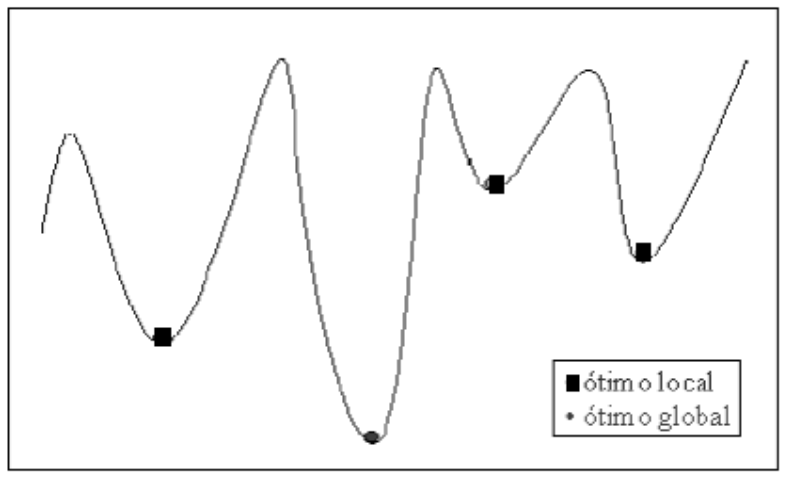
\includegraphics[scale=0.55]{imagens/problemaOtimizacao.png}
\\ \textbf{\footnotesize Fonte: \cite{timoteo2005desenvolvimento}}
\end{figure}
	
Segundo \cite{steiglitz1982combinatorial}, os problemas de otimização são divididos em duas categorias, problemas com variáveis contínuas e problemas com variáveis discretas. Problemas com variáveis discretas também podem ser conhecidos como Problemas de Otimização Combinatória (POC).\par

Conforme cita \cite{raupp2003introduccao}, o problema de otimização combinatória pode ser denominado como a ação de maximizar ou minimizar uma função objetiva de diversas variáveis sujeita a um conjunto de restrições, dentro de um contexto.\par

De acordo com \cite{opac-b1092847} problemas do tipo POC tratam do estudo matemático para encontrar agrupamentos, arranjos ou a seleção ótima de objetos discretos, logo, não permitindo, a utilização de métodos clássicos de otimização contínua para sua resolução.\par


Segundo \cite{golbarg2000otimizaccao} a ocorrência de problemas de otimização combinatória podem acontecer em diversas áreas, projetos de sistemas de distribuição de energia elétrica, posicionamento de satélites, roteamento ou escalonamento de veículos, sequenciamento de genes e DNA, classificação de plantas e animais.\par

De acordo com \cite{deleonardo} em problemas de otimização combinatória, cujo universo de dados é grande e existe um grande número de combinações, o que torna inviável a análise de todas soluções possíveis em um tempo adequado, utilizamos as heurísticas, também conhecidas como algoritmos heurísticos, que são métodos que compõem uma gama de soluções para problemas de otimização combinatória.

\secao{Heurística}

O termo heurística é derivado do grego \textit{heuriskein}, o que significa descobrir ou achar. De acordo com \cite{timoteo2005desenvolvimento} o significado da palavra em pesquisa operacional vai um pouco além da raiz etimológica. Segundo \cite{steiglitz1982combinatorial}, heurísticas são consideradas métodos de aproximação ou métodos de busca de solução, deve se levar em consideração que não exista uma garantia formal de seu desempenho e uma garantia de que estas heurísticas que iram encontrar uma solução. As heurísticas, apesar de não garantirem encontrar a solução ótima para um problema, procuram por soluções consideradas de boa qualidade em um tempo computacional razoável.\par

Segundo \cite{evans1992optimization} heurísticas são necessárias para implementação de problemas NP Difícil, caso deseje-se resolver tais problemas em um tempo  razoável.\par

Ressalta-se que dentre as heurísticas, as chamadas meta-heurísticas, merecem especial atenção pois adotam técnicas para amenizar, a dificuldade que os métodos heurísticos têm de escapar dos ótimos locais. As meta-heurísticas podem partir em busca de regiões mais promissoras no espaço de soluções, alem disto, as meta-heurísticas possuem grande abrangência, podendo ser aplicada à maioria dos problemas de otimização combinatória.\cite{nascimento2005aplicaccao}\par

As meta-heurísticas surgiram como uma alternativa para amenizar a dificuldade que os métodos heurísticos tem de escapar dos chamados ótimos locais.\cite{nascimento2005aplicaccao}

Segundo \cite{adrianocesar} uma heurística é a instanciação de uma meta-heurística, ou seja, a aplicação da mesma em um problema específico de otimização.\par

Como exemplos de meta-heurísticas temos Busca Tabu (\textit{Tabu Search}), Otimização por Colônias de Formigas (\textit{Ant Colony Optimization}), Recozimento Simulado (\textit{Simulated Annealing}) e Algoritmo Genético (\textit{Genetic Algorithm}).\par

\subsecao{Busca Tabu}

Busca tabu (BT) é uma meta-heurística adaptativa, que utiliza uma estrutura de memória através de uma lista, contendo um histórico de evolução para evitar que o processo de busca forme ciclos, ou seja, o retorno a um ótimo local previamente visitado \cite{souza2000} , \cite{armentanointroduccao} e \cite{subramanian2006aplicaccao}.\par


Segundo \cite{subramanian2006aplicaccao} BT foi desenvolvida por \cite{glover1986future} com o objetivo de encontrar soluções para problemas de programação linear. Ao formalizar a técnica, o autor publicou uma serie de trabalhos envolvendo diversas aplicações da meta-heurística. \par

Basicamente o funcionamento do BT a feito partir da definição de uma população inicial ${S_0}$, o algoritmo explora cada iteração, de um subconjunto V da vizinhança N(S) da solução corrente S. O membro S’ de V com melhor valor nessa região segundo a função f(.) torna-se a nova solução corrente mesmo que S’ seja pior que S isto é, que f(S’) $>$ f(S) para um problema de minimização\cite{souza2000}. A figura 2 representa o pseudocódigo do algorítimo da Busca Tabu.

Segundo \cite{armentanointroduccao}  o algorítimo tem um intensivo uso de memória o que é uma característica essencial deste método. Para o autor o uso da memória pode ajudar a intensificar a busca em regiões com grande chances de se encontrar o resultado, ou até mesmo, diversificar a busca através de regiões inexploradas.
\begin{figure}[!htb]
\caption[Representação do pseudocódigo do algorítimo da Busca Tabu]{Representação do pseudocódigo do algorítimo da Busca Tabu}
\label{fig:figura2}
\centering
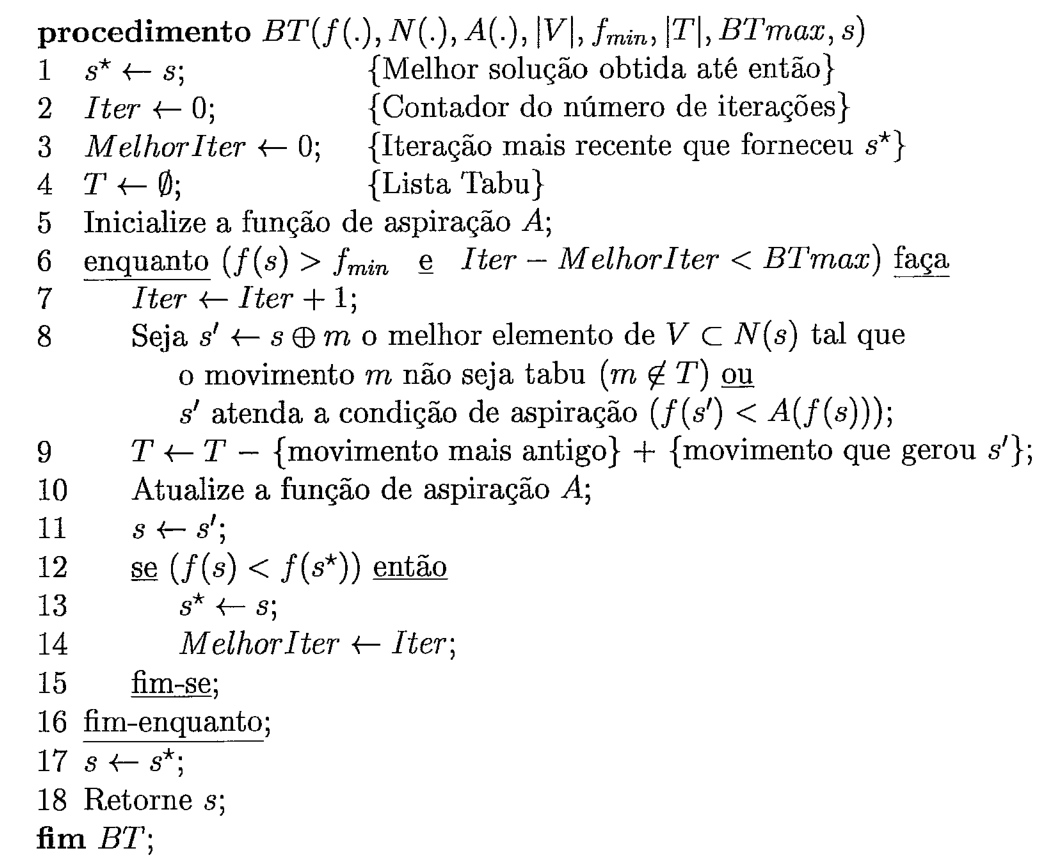
\includegraphics[scale=0.50]{imagens/representacaoBuscaTabu.png}
\\ \textbf{\footnotesize Fonte: \cite{souza2000}}
\end{figure}

De acordo com \cite{armentanointroduccao}  devemos adotar alguns procedimentos para que o processo de busca tenha um melhor resultado, listas tabu dinâmicas, passagens por regiões planas, intensificação, diversificação,\textit{path relinking}. Listas tabu dinâmicas tem como objetivo evitar que o algorítimo entre em processo de ciclo.Passagens por regiões planas pode levar o algorítimo a pensar que não existem melhoras significativas na qualidade das soluções e atingir o critério de parada, para evitar esta situação é necessário aumentar o tamanho da lista tabu enquanto o algorítimo estiver passando pela região plana e voltar a reduzir quando houver mudança no valor da função objetiva.Intensificação são técnicas utilizadas para concentrar os esforços da pesquisa em regiões consideradas promissoras. Diversificação é uma técnica que utiliza memória de longo prazo para redirecionar a pesquisa para regiões que ainda não foram suficientemente exploradas. PathRelinking trada ta intensificação de incorporar atributos de soluções de boa qualidade (chamadas de soluções elite), em seguida explora caminhos que contenham uma ou mais soluções de elite.

Ainda segundo \cite{armentanointroduccao} uma característica importante do método é que a solução final tem pouca ou nenhuma dependência da escolha feita para a solução inicial, isso graças aos mecanismos implementados pelo método, que fogem de ótimos locais.

\subsecao{Recozimento Simulado}

Técnica de busca local probabilística, proposta originalmente por \cite{kirkpatrick1983optimization}, que se fundamenta em uma analogia com a termodinâmica, ao simular o 
resfriamento de um conjunto de átomos aquecidos.\par 

Isto é, conforme \cite{noronha2003abordagem} em analogia a física da matéria: levando um cristal a sua temperatura de fusão, as moléculas estão desordenadas e se agitam livremente. Ao resfriar-se a amostra de maneira infinitamente lenta, as moléculas vão adquirir a estrutura cristalina estável que tem um nível de energia mais baixo possível.\par 

Segundo \cite{souza2002experiencias} o processo se inicia com um membro qualquer do espaço de soluções, normalmente gerado aleatoriamente, e seleciona um de seus vizinhos randomicamente. Se este vizinho for melhor que o original ele é aceito e substitui a solução corrente. Se ele for pior por uma quantidade ∆, ele é aceito com uma probabilidade e -∆/T , onde T decresce gradualmente conforme o progresso do algoritmo. Esse processo é repetido até que T seja tão pequeno que mais nenhum movimento seja aceito. A melhor solução encontrada durante a busca é tomada como uma boa aproximação para a solução ótima. Originalmente, Simulated Annealing foi derivado de simulações em termodinâmica e por esta razão o parâmetro T é referenciado como temperatura e a maneira pela qual ela é reduzida é chamada de processo de resfriamento.


A figura 3 representa o pseudocódigo do algoritmo Simulated Annealing.

\begin{figure}[!htb]
\caption[Representação do pseudocódigo do algorítimo Simulated Annealing]{Representação do pseudocódigo do algorítimo Simulated Annealing}
\label{fig:figura2}
\centering
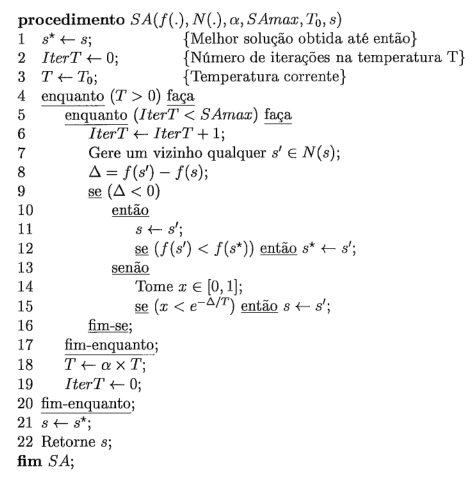
\includegraphics[scale=0.55]{imagens/representacaoSimulatedAnnealing.png}
\\ \textbf{\footnotesize Fonte: \cite{souza2002experiencias}}
\end{figure}

Conforme \cite{aarts1988simulated} a analogia com a otimização (combinatória ou não) é bastante direta. Os estados da matéria são as soluções realizáveis, a quantidade objetiva substitui a energia, os estados metaestáveis da matéria sendo ótimos locais e a estrutura cristalina corresponde ao ótimo global.\par 



\subsecao{Algoritmos genéticos}

%o que é 

De acordo com \cite{goldberg1989genetic} algoritmos genéticos são baseados na teoria da evolução das espécies elaborada por \cite{darwin1968origin} utilizando os conceitos da biológia tais como genes, individuo, população, cromossomos, cruzamento, mutação e seleção. Estes algoritmos foram introduzidos por \cite{holland1975adaptation} para resolver os problemas chamados \textit{timetabling}.

Para entender melhor \cite{mitchell1998introduction} descreve os principais termos biológicos necessários para o funcionamento dos algoritmos genéticos. Gene se trada de uma característica particular de um cromossomo. Um cromossomo é composto por um ou mais genes, pode se dizer também que é uma sequencia de genes que será caracterizada como a solução do problema. \textit{Fitness} significa a aptidão do indivíduo em um determinado ambiente. Individuo é a combinação do cromossomo mais o \textit{fitness} calculado através da função objetiva. População é um grupo de indivíduos. Geração se trata de cada interação do algoritimo.\par

Em seu trabalho \cite{lucas2000algoritmos} descreve algoritmos genéticos da seguinte forma. São algoritmos que trabalham sobre uma população, através de uma função de adaptação, para que aconteça a evolução. Primeiramente é inicializada uma população, logo após iram acontecer os processos de seleção, reprodução também conhecida como \textit{crossover} e mutação, os mesmos ocorreram a cada geração até que os critérios de parada aconteçam. Também afirma que os termos utilizados pertencem à tradição existente no meio da computação evolutiva de utilizar, com certa liberdade os termos da biologia.

Segundo \cite{oliveira2005algoritmo}, o processo de evolução executado por um algoritmo genético corresponde a um procedimento de busca no espaço de soluções potenciais para o problema e, como enfatiza \cite{michalewicz1996evolutionary}, esta busca requer um equilíbrio entre dois objetivos aparentemente conflitantes: a procura das melhores soluções na região que se apresenta promissora ou fase de intensificação e a procura de outra região ou exploração do espaço de busca, também conhecida como diversificação.\par

\begin{figure}[!htb]
\caption[Estrutura funcional de um algoritmo genético típico]{Estrutura funcional de um algoritmo genético típico}
\label{fig:ag}
\centering
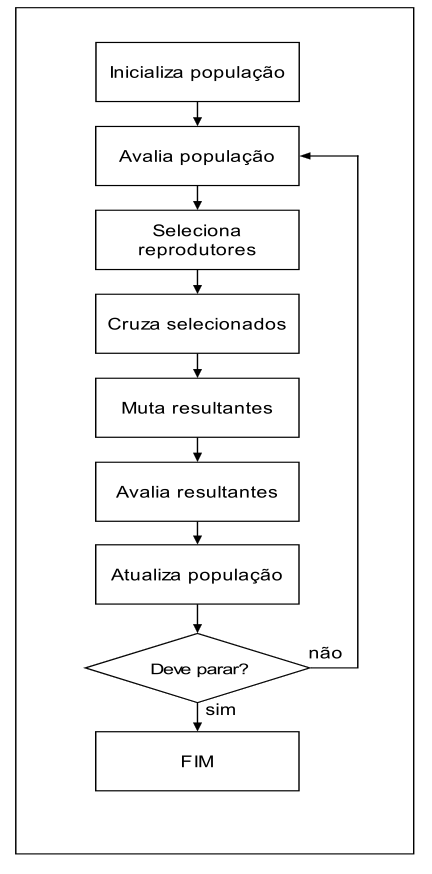
\includegraphics[scale=0.6]{imagens/ag.png}
\\ \textbf{\footnotesize Fonte: \cite{de1999introduccao}}
\end{figure}

%falar sobre população inicial

A Figura~\ref{fig:ag} trata de uma estrutura funcional típica de um algorítimo genético, \cite{de1999introduccao} cita em seu trabalho que o primeiro passo a ser tomado é a geração de uma população inicial, que é formada através de métodos aleatórios para gerar os indivíduos, assim teremos uma biodiversidade na população. Durante o processo evolutivo todos indivíduos da população são avaliados e cada um deles recebe o seu \textit{fitness}, o que representa a qualidade da solução representada por ele.\par

%falar sobre seleção

Segundo \cite{lobo2005soluccao} existem vários métodos para selecionar indivíduos para execução dos operadores genéticos, em seu trabalho o autor apresenta os seguintes métodos. Seleção por roleta é um método tradicional, para cada indivíduo é atribuído um espaço na roleta sendo o tamanho proporcional ao valor da aptidão do individuo. Esta roleta gira N vezes onde N é o numero do tamanho da população, selecionando assim os pais para próxima geração. Seleção por torneio são selecionados X indivíduos da população onde X é um valor aleatório anterior e escolhidos os dois que que contêm o maior valor de aptidão no caso os país, segundo o autor este método é o mais utilizado, pois oferece a vantagem de não exigir que a comparação seja feita entre todos os indivíduos da população.\par

%falar sobre operadores genéticos.

De acordo com \cite{goes2005otimizaccao} os principais operadores genéticos, utilizados ao se desenvolver algorítimos genéticos são inversão, mutação e \textit{crossover}, são responsáveis em realizar transformações nos indivíduos da população mas cada um possui suas diferentes funções dentro do algorítimo.\par
Inversão é um operador que modifica a genética de um gene ele é fundamental para garantir a biodiversidade da população, ainda segundo \cite{goes2005otimizaccao} o operador mutação  desenvolve o mesmo papel que o operador inversão, o mesmo cita que vários autores consideram inversão e mutação como o mesmo operador genético e também afirmam que são os operadores mais importantes e optam por trabalhar somente com estes operadores. Estes operadores são fundamentais para o desenvolvimento de algorítimos genéticos por evitarem a convergência prematura da solução, ou seja, quando uma população se estabiliza com uma adaptação pouco adequada, podemos dizer então que, um super-indivíduo domina o processo seletivo de tal forma que não é possível gerar filhos melhores, este mesmo super-indivíduo transmite suas características para toda a população.\par

O operador cruzamento também conhecido como \textit{crossover} é um operador genético onde é selecionado um ponto de corte produzindo duas cabeças e duas caldas após isto é realizada a troca das caldas dos pais criando dois filhos contendo material genético similares aos dos pais a figura~\ref{fig:pontoCorteAG} mostra onde é realizado o ponto de corte como ficam os filhos criado após a troca das caldas \cite{de1999introduccao}.

\begin{figure}[!htb]
\caption[Ponto de corte \textit{crossover}]{Ponto de corte \textit{crossover}}
\label{fig:pontoCorteAG}
\centering
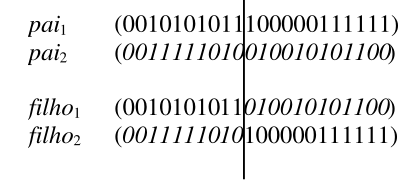
\includegraphics[scale=0.6]{imagens/crossoverAG.png}
\\ \textbf{\footnotesize Fonte: \cite{de1999introduccao}}
\end{figure}

No artigo apresentado pelos autores \cite{de1999introduccao} o elitismo é descrito como um operador genético que foi proposto por \cite{DeJong} em seu trabalho, que é dos pioneiros sobre algorítimos genéticos. Uma vez que os melhores indivíduos, de acordo com a função objetiva, podem ser perdidos entre uma geração e outra devido ao corte do \textit{crossover} e a execução da mutação, torna-se interessante transferir o melhor indivíduo para a próxima geração, o nome dado para está estratégia se chama elitismo uma técnica muito utilizada ao se desenvolver AGs. Os autores apresentam gráficos que mostram o desempenho da utilização do operador, segundo os mesmo quando se é utilizado o operador fica claramente observado que, com o uso do elitismo o algorítimo encontra a solução mais rápida, do que quando não ocorre a utilização do operador.

Segundo \cite{hamawaki2011geraccao} e \cite{oliveira2005algoritmo} algoritmos genéticos são eficientes para encontrar soluções ótimas ou quase ótimas, pois as limitações são minimas dos demais métodos de busca tradicionais. Ainda segundo \cite{oliveira2005algoritmo}, os algoritmos genéticos têm se mostrado ferramentas poderosas para resolver problemas onde o espaço de busca é muito grande e os métodos convencionais se mostraram ineficientes.\par


\secao{TimeTabling}

Segundo \cite{kripkasimulated} os problemas de programação de horários (PPH), também conhecidos como \textit{TimeTabling}, são os problemas que mais se destacam nas organizações acadêmicas. De acrodo com \cite{schaerf1999survey} estes problemas são divididos em três categorias \textit{school timetabling}, \textit{course timetabling} e \textit{examination timetabling}.\par

\textit{School TimeTabling}: Se trata basicamente da geração de horários semanais, em escolas de segundo grau, onde deve-se evitar os choques entre os horários das disciplinas e que cada professor receba apenas uma turma para cada horário. Neste caso o aluno recebe um número fixo de disciplinas a serem cursadas.\par

\textit{Course TimeTabling}: Diz respeito à alocação de aulas de uma universidade típica. Neste problema os alunos podem escolher as matérias em que vão se matricular, portando o problema tem como objetivo minimizar os possíveis choques entre as disciplinas, professores e horários disponibilizados pela instituição de ensino.\par

\textit{Examination TimeTabling}: Aborda o problema de programação de horários dos exames da instituição, de maneira que, disciplinas que tenham alunos em comum, distanciem o máximo possível as datas dos exames.\par

Segundo \cite{pinheiro2001ambiente} o problema de programação de horários vem sendo abordado desde a década de 60, sendo que os primeiros trabalhos a se destacarem foram realizados na década de 80.\par

O Problema de Alocação de Salas (PAS) também conhecido como \textit{Classroom Assignment} é tratado como parte do problema de programação de cursos universitários \textit{course timetabling}. Segundo \cite{marinho2005heuristicas} varias instituições universitárias se deparam com o PAS durante o início de cada semestre letivo, este problema é considerado NP-Difícil por \cite{even1975complexity} e \cite{carter1992classroom}, com isto, a determinação da solução ótima do problema, em um período de tempo aceitável se torna uma tarefa difícil.\par
Segundo \cite{kripkasimulated} o problema deve considerar que as disciplinas dos cursos universitários já tenham seus horários de início e de término definidos. O problema se resume então na alocação das disciplinas às salas desta universidade respeitando os horários destas disciplinas e as demais restrições exigidas.

Segundo \cite{souza2000} boa parte das universidades ainda resolvem este problema de forma manual, o que torna o processo árduo e demorado, podendo levar vários dias para ser concluído.\par

Uma vez que é de extrema dificuldade encontrar a solução ótima do PAS em tempo razoável, este problema é normalmente tratado através de técnicas heurísticas, que apesar de não garantirem encontrar a solução ótima do problema, são capazes de retornar uma solução de qualidade em um tempo adequado.\cite{nascimento2005aplicaccao}.Segundo \cite{even1975complexity} o PAS pertence a classe de Problemas de Otimização Combinatória (POC).\par


\secao{Trabalhos Relacionados}
trabalho do marinho que usa tabu.
trabalho da silvia que usa Recozimento Simulado (Simulated Annealing).
trabalho da leonardo que usa Algoritmos Genéticos (AG).
achar algum trabalho que utiliza o algoritimo das formigas.
falar porque o trabalho do cara se assemelha ao meu trabalho.
%
\capitulo{METODOLOGIA}

\iniciocapitulo
A resolução deste trabalho está dividida nas seguintes partes instalação do ambiente, análise e algorítimo.\par

A implementação do sistema se deve primeiramente a configuração do ambiente para o início do desenvolvimento os seguintes passos devem ser tomados para que o ambiente seja reproduzido novamente. Primeiramente deve se instalar o SGBD PostgreSQL, logo em seguida deve se instalar o JAVA 7 em sua maquina, para validar a instalação deve-se executar o seguinte comando "java -version && javac -version" a mensagem descrita na figura XX deve ser mostrada.

\begin{figure}[!htb]
\caption[Versão Java]{Versão Java}
\label{fig:figura2}
\centering
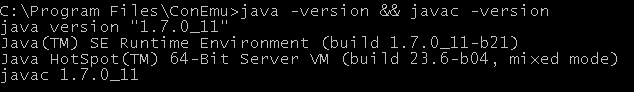
\includegraphics[scale=0.8]{imagens/mensagemJava.png}
\\ \textbf{\footnotesize Fonte: Autor}
\end{figure}


Após a instalação do java deve-se instalar o framework Play! seguindo os passos encontrados no site \cite{play} para validar a instalação do Play! deve se executar o comando "play version" e o \textit{prompt} de comando deve retornar a mensagem conforme mostra a figura figura XX.

\begin{figure}[!htb]
\caption[Versão Framework]{Versão Framework}
\label{fig:figura2}
\centering
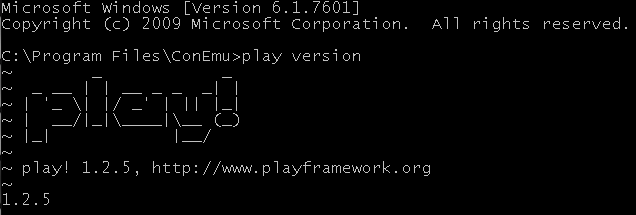
\includegraphics[scale=0.8]{imagens/mensagemPlay.png}
\\ \textbf{\footnotesize Fonte: Autor}
\end{figure}

Uma vez que o ambiente já está configurado devemos inciar um projeto no framework instalado através do comando "play new nomeDoProjeto", a partir dai é possível escolher IDE que será utilizada.

Foi criado um \textit{script} para criação do banco de dados e população inicial das informações como, prédios, salas, turnos, horários, e disciplinas com informações que são necessárias em todo inicio de semestre na instituição de ensino escolhida.

PQ do algoritimo genetico
segundo renand dupas a escolha de algoritimoes geneticos se dá através de uma comparação com outras técnicas e através disso de uma evidenciação das vantagens de sua utilização , logo o algoritimo genetico foi escolhido para este trabalho.

População inicial = --UMA NOVA ABORDAGEM PARA AUMENTAR A DIVERSIDADE.pdf

modelo matematico ----APLICAÇÃO DE MODELO MATEMÁTICO, ABORDAGEM HEURÍSTICA E MÉTODO MISTO NA OTIMIZAÇÃO DA PROGRAMAÇÃO DE HORÁRIO DOS PROFESSORESTURMAS.pdf

restrições do problema e modelo matematico http://www.dcc.ufla.br/infocomp/artigos/v4.3/art08.pdf

Foi realizada uma análise dos requisistos atravez de entrevista com o steakholder, após as entrevistas a modelagem de dados foi realizada de acordo com a demanda do projeto, para o desenvolvimento destes diagramas foi utilizadas a UML (Universal Modeling Language). Os seguintes diagramas foram desenhados, diagrama de caso de uso, diagrama de classe e diagrama de entidade relacionamento. Foram escolhidos os seguintes diagramas para que o sistema tenha uma documentação minima tendo em vista que o foco do trabalho é a resolução do problema de timetable através da utilização do algoritimo genetico.

Por se tratar de um sistema complexo, antes de iniciar a implementação do sistema
fez-se necessário a sua modelagem. Segundo Elmasri & Navathe (2005) as metodologias
de modelagem de dados de objetos como UML (Universal Modeling Language –
Linguagem de Modelagem Universal) estão se tornando cada vez mais populares no
projeto e engenharia de software. Essas metodologias vão além do projeto de um banco de
dados, especificando o projeto detalhado dos módulos de software e suas interações,
utilizando vários tipos de diagramas.\par

\secao{Ferramentas Utilizadas}

Este trabalho conta com a utilização de tecnologias proprias para o desenvolvimento de sistemas web, foram utilizadas as seguintes ferramentas: Para SGBD foi o utilizado PostgreSQL; No back-end foi utilizado Java e o \textit{framework Play!}; No front-end as tecnologias utilizadas foram HTML, CSS, JavaScript e \textit{framework AngularJS} e a IDE utilizada \textit{Eclipse}.\par



\subsecao{Sistema de Gerenciamento de Banco de Dados}

O SGBD escolhido foi o PostgreSQL pelo fato de ser uma ferramenta open-source e que trabalha perfeitamente com o framework escolhido Play!, uma vez que utilizado em projetos anteriores não foram apresentados conflitos entre o framework e o SGBD. A seguir pode ser notar que é uma ferramenta robusta e que tem visão no mercado internacional.\par

O PostgreSQL é um poderoso sistema gerenciador de banco de dados objeto-relacional de código aberto.  Tem mais de 15 anos de desenvolvimento ativo e uma arquitetura que comprovadamente ganhou forte reputação de confiabilidade, integridade de dados e conformidade a padrões.  Roda em todos os grandes sistemas operacionais. É totalmente compatível com ACID, tem suporte completo a chaves estrangeiras, junções (JOINs), visões, gatilhos e procedimentos armazenados (em múltiplas linguagens).  Inclui a maior parte dos tipos de dados do ISO SQL:1999, incluindo INTEGER, NUMERIC, BOOLEAN, CHAR, VARCHAR, DATE, INTERVAL, e TIMESTAMP.  Suporta também o armazenamento de objetos binários, incluindo figuras, sons ou vídeos.  Possui interfaces nativas de programação para C/C++, Java, .Net, Perl, Python, Ruby, Tcl, ODBC, entre outros, e uma excepcional documentação.\cite{postgresql}



Para a resolução do problema de timetable foi escolhido o algoritimo genetico, a escolha do algoritimo foi devida a grande utilização do mesmo para resolução de problemas do tipo NP-dificil que foram encontrados na literatura.
\par




\subsecao{Ferramentas Back-end}

Foi escolhida uma linguagem de programação Java por ser orientada a objeto. Tambem foi escolhido o \textit{Play! framework}, para que o desenvolvimento aconteça de forma mais rápida, fácil e eficiente.\par

%Java
Java foi criada pela Sun Microsystems para desenvolver inovações tecnológicas em 1992, time liderado por James Gosling. O Java utiliza do conceito de máquina virtual, onde existe, entre o sistema operacional e a aplicação, uma camada extra responsável por \"traduzir\" - mas não apenas isso - o que sua aplicação deseja fazer para as respectivas chamadas do sistema operacional, onde ela está rodando no momento. Sua aplicação roda sem nenhum envolvimento com o sistema operacional, sempre conversando apenas com a JVM - Java Virtual Machine \cite{caelum}.\par

Em 2009 a Oracle comprou a Sun, fortalecendo a marca. A Oracle sempre foi, junto com a IBM, uma das empresas que mais investiram e fizeram negócios através do uso da plataforma Java. Em 2011 surge a versão Java 7 com algumas pequenas mudanças na linguagem \cite{caelum}.\par

%-----Play! Framework

The Play! É um moderno framework MVC de alta produtividade, que utiliza Java e Scala para o desenvolvimento web, open-source , utiliza templates, hibernate e JUnit  em sua arquitetura. Existe duas versões do framework Play! 1 e Play2! este trabalho utiliza a versão 1 do framework\cite{playframework}.\par


\subsecao{Ferramentas Front-end}

As ferramentes de Front-end descritas abaixo, foram escolhidas devida a gande utilização na web grande parte dos sites contem HTML, CSS ou JavaScript em algum trexo de seu código, foi escolhido tambem o framework AngularJS para que o desenvolvimento ocorra de maneira agil e mais rapida.\par

%HTML
HTML que é defindo por (\textit{HyperText Markup Language}) ou linguagem de marcação, é uma linguagem que é utilizada no desenvolvimento de paginas web \cite{html}.\par

%css
Cascading Style Sheets (CSS) é uma tecnologia utilizada para adicionar estilos como cores, fontes, espaçamentos em documentos escritos em uma linguagem de marcação como exemplo o HTML \cite{css}.\par

%JAVASCRIPT

JavaScript é uma linguagem de script utilizada no desenvolvimento de paginas na web, atualmente é a principal linguagem para programação client-side em navegadores web. Todas as paginas de HTML modernas estão usando JavaScript para adicionar funcionalidades e para se comunicar com os webServers\cite{javascript}.\par

Angularjs é um \textit{framework JavaScript} construido e mantido pelo grupo de engenheiros do Google, ele usa o HTML como uma \textit{template engine}, tudo isso no intuito de fornecer uma solução completa para o cliente-side de sua aplicação. Além disso tem total compatibilidade com as bibliotecas javascript mais utilizadas, como jQuery. É um novo conceito para desenvolvimento de web apps client-site.\cite{angularjs}\par

\subsecao{IDE}

O Eclipse é uma IDE (\textit{integrated development environment}). Diferente de uma RAD(\textit{Rapid Application Development}), onde o objetivo é desenvolver o mais rápido possível através do arrastar-e-soltar do mouse, onde montanhas de código são gerados em background, uma IDE te auxilia no desenvolvimento, evitando se intrometer e fazer muita mágica \cite{caelum}.\par

O Eclipse é a IDE líder de mercado. Formada por um consórcio liderado pela IBM, possui seu código livre. A última versão é a 4.3, mas com qualquer versão posterior a do 3.1 você terá suporte ao Java 5, 6 e 7 \cite{caelum}.\par

Está IDE foi escolhida devido ao grande reconhecimento mundial, por sua eficiencia ao se trabalhar com a linguagem de programação Java, por ser open-source e pela existencia de varias ferramentas criadas pela comunidade, para o auxilio no desenvolvimento de softwares.\par
%\capitulo{SISTEMA DESENVOLVIDO}

Será desenvolvido um sistema que otimiza a alocação das salas facilizando a vida do gerente. Por se tratar de um problema especifico fica dificil encontrar tecnlogias disponiveis para a resolução do problema sendo assim necessario o atendimento de um sistema que atenda todas as necessisdades exigidas.

\secao{Modelagem}

Arrumar referencia.\par

Segundo Booch et al. (2001) a modelagem de um diagrama de caso de uso é uma
técnica usada para descrever e definir os requisitos funcionais de um sistema. Para sistemas
que possuem um número elevado de funcionalidades, a construção destes diagramas visa
facilitar o entendimento do problema, a documentação do que será desenvolvido bem
como facilita o próprio desenvolvimento.


\subsecao{Diagramas de entidade relacionamento}

Arrumar referencia.\par
Por se tratar de uma aplicação de banco de dados, a modelagem de dados foi
também construída. Segundo Elmasri & Navathe (2005) a modelagem conceitual é uma
fase muito importante no planejamento de uma aplicação de um banco de dados bem
sucedida.
Ainda segundo Elmasri & Navathe (2005), o modelo relacional representa o banco
de dados como uma coleção de relações. Informalmente, cada relação se parece com uma
tabela de valores.
Na Figura 3.8 tem-se o diagrama para o esquema do banco de dados relacional do
sistema. Cada tabela é chamada de relação e cada cabeçalho de coluna é conhecido como
atributo. Os atributos sublinhados em cada tabela indicam a chave-primária e a indicação
“(FK)” exibe a chave-estrangeira em cada relação.

\begin{figure}[!htb]
\caption[Diagrama de componetes do sistema xxx]{Diagrama de componetes do sistema xxx}
\label{fig:figura1}
\centering
\includegraphics{images/diagramaComponentes.png}
\\ \textbf{\footnotesize Fonte: Desenvolvido pelo autor}
\end{figure}


\subsecao{Diagramas de caso de uso}


A Figura 3.4 descreve todas as funcionalidades que o usuário de perfil
“Administrador” poderá executar na ferramenta.


\begin{figure}[!htb]
\caption[Diagrama de componetes do sistema xxx]{Diagrama de componetes do sistema xxx}
\label{fig:figura1}
\centering
\includegraphics[scale=0.8]{images/diagramaComponentes.png}
\\ \textbf{\footnotesize Fonte: Desenvolvido pelo autor}
\end{figure}

Já a Figura 3.5 apresenta as funcionalidades que o usuário de perfil Consulta pode
executar. A seta partindo do usuário Administrador indica que este pode executar qualquer
funcionalidade que o usuário Consulta tem acesso.

\begin{figure}[!htb]
\caption[Diagrama de componetes do sistema xxx]{Diagrama de componetes do sistema xxx}
\label{fig:figura1}
\centering
\includegraphics{images/diagramaComponentes.png}
\\ \textbf{\footnotesize Fonte: Desenvolvido pelo autor}
\end{figure}



\subsecao{Diagramas de classe}

Segundo Booch et al. (2001), Diagrama de Classes demonstram a estrutura estática
das classes de um sistema, onde estas representam as “coisas” que são gerenciadas pela
aplicação modelada. Ainda segundo Booch et al. (2001), uma classe num diagrama pode
ser diretamente implementada utilizando-se uma linguagem de programação orientada a
objetos, no caso deste trabalho, a Linguagem Java.
A partir da Figura 3.7 pode-se observar as classes manipuladores do sistema. Elas
estão identificadas, descritas com seus métodos e relacionadas entre si. Geralmente um
sistema possui mais de um diagrama, pois nem todas se encaixam em um diagrama
específico.

\begin{figure}[!htb]
\caption[Diagrama de componetes do sistema xxx]{Diagrama de componetes do sistema xxx}
\label{fig:figura1}
\centering
\includegraphics{images/diagramaComponentes.png}
\\ \textbf{\footnotesize Fonte: Desenvolvido pelo autor}
\end{figure}
%==============================================%

\secao{Algoritimo Genético}


O primeiro passo a ser dado para o desenvolvimento do algoritimo é o pleno conhecimento do problema e a ligação entre os termos utilizados na biologia com os itens do problema proposto anteriormente. Foram utilizadas varias fontes para o desenvolvimento do trabalho, porem foram feitas modificação para que o modelo tratado por outros autores funcionasse como necessario.\par

Para o melhor entendimento dos passos tomados durante a interpretação do problema e da sua ligação com o algoritmo genetico será criado um pequeno ambiente de alocação. Este ambiente contem as seguintes propriedades, três salas, seis horarios, sete dias da semana, cinco discplinas, e 9 relacionamentos de obrigatoriedade entre discplina e horário.\par

\begin{figure}[!htb]
\caption[Representação do ambiente]{Representação do ambiente}
\label{fig:figura1}
\centering
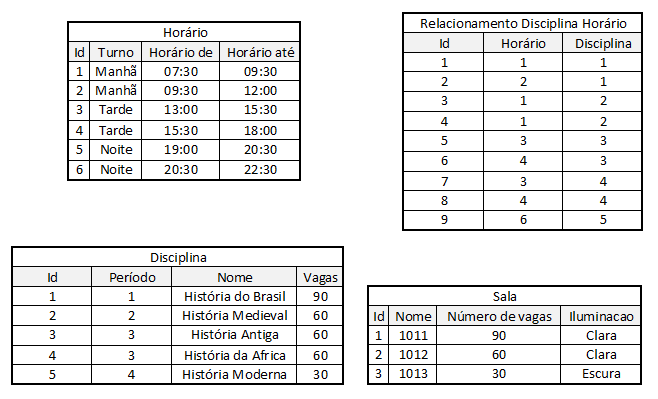
\includegraphics{imagens/representacaoAmbiente.png}
\\ \textbf{\footnotesize Fonte: Desenvolvido pelo autor}
\end{figure}

\subsecao{Individuo}

	Alguns trabalhos tratam cromossomos e inidviduos pela mesma representação biologica, neste caso cromosso neste trabalho o termo cromossomo se refere a segquencia de genes e o termo Indiviuo será a combinação de cromossomo e fitness.\par

	O termo Gene representa uma combinação de quatro variaveis Sala, Dia da Semana, Horario, e o relacionamento entre Disciplina Horario. As três primeiras variaveis são fixas e não podem ser nulas pois o conjunto de Genes forma um cromossomo que é a alocação de todas as discplinas em horarios diferentes.\par

	Um Gene com o relacionamento Disciplina Horario igual a nulo, representa um horario vago, como exemplo podemos descrever a seguinte situação, {sala:"3001", diaDaSemana:"1", horario:"3", disciplinaHorario:"null"} mostra que nos determinados parametros não existe nenhuma sala alocada.\par

	Um cromossomo é uma seguencia de genes o que representa uma alocação completa que engloba todas as salas, todos os dias da semana, e todos os horarios disponiveis para alocação de disciplinas. Uma vez que este valor não é variavel temos um cromossomo com um valor fixo, que serão inseridos os horarios disponiveis para alocação das disciplinas.\par


	Por fim individuo é a combinação do cromossom e a poutnação adquirida após a execuação do metodo de calculo de fitness.

\subsecao{Populacao}
	
	População é o conjunto de individuos

\subsecao{Populacao Inicial}

\subsecao{Nova População}

\subsecao{Definição da função objetivo}
Somatorio disso

Para o calculo do fitness foram definidos pesos para modelagem da função, estes pesos podem ser configurados de acordo com a necessidade da alocação.

Graduação alocada ganha 05 de peso

Pós graduação alocada ganha 03 de peso

Periodos na mesma sala cada um ganha 05 de peso * o numero do periodo

Quanditadade de vagas igual a da sala 05 de peso

não optativa ganha 5

optativa ganha 3

iliminacao atendida 5

Criar a função matematica com as legendas conforme o trabalho 117.pdf

Falar o numero de salas, o numero de horarios, o numero de curos o numero de colegiados o numero de periodos o numero de disciplinas para cada colegiado.......

restrições 


falar um pouco das restrições e enumeralas

As disciplinas não podem ser alocadas em horarios direfentes dos que já foram pré definidos pelo colegiado.

As discplinas devem ter apenas a quantidade de alocações necessarias.

As disciplinas devem respeitar a capacidade da sala.

As diciplinas não optativas tem preferencia de alcação na mesma sala.

Preferencias por salas claras ou escuras

Restrição 1 


Fitness

Para se iniciar o calculo do fitness são verificados todos os horarios já alocados somando os pesos se adequados.

para cada gene

se tem horario alocado 

horario bate

capacidade da turma

turma graduacao

optativa

iluminacao

soma tudo

fim se tem alocação

soma tudo

fim para cada gene

Calculo do fitness01 somatatoriox100/colocar algum valor  para dividir não sei ainda

calculo fitness02 penaliza disciplinas com mais alocação do que se deve

para cada gene 

para cada disciplina 

soma

fim

Calculo fitness02 -= fitnes01 x (1 - (total alocados - total necessario/ dividir pelo numero possivel de alocações))
fim

calculo fitness03 penalidade por capacidade

para cada gente

se a sala tiver capacidade diferente

fim

calculo fitness03 = fitness02 x (1 - (numero de erros /  numero de possiveis alocações )))


calculo fitness04 preferencias clara ou escura

para cada gene 

se tiver com o optativo errado 

fim	

calculo fitness04 = fitness03 x (1 - (numero de erros /  numero de possiveis alocações )))


O fitness04 é o resultado final

\subsecao{Seleçao por torneio}


\subsecao{Operadores Geneticos}
elitismo
crossover
mutacao


\capitulo{SISTEMA DESENVOLVIDO}

Será desenvolvido um sistema que otimiza a alocação das salas facilizando a vida do gerente. Por se tratar de um problema especifico fica dificil encontrar tecnlogias disponiveis para a resolução do problema sendo assim necessario o atendimento de um sistema que atenda todas as necessisdades exigidas.

\secao{Modelagem}

\subsecao{Diagramas de caso de uso}

Arrumar referencia \par

Segundo Booch et al. (2001) a modelagem de um diagrama de caso de uso é uma técnica usada para descrever e definir os requisitos funcionais de um sistema. Para sistemas que possuem um número elevado de funcionalidades, a construção destes diagramas visa facilitar o entendimento do problema, a documentação do que será desenvolvido bem como facilita o próprio desenvolvimento.\par

A Figura XX descreve todas as funcionalidades que o sistema possui, essas funcionalidades foram dividias em 2 atores "Gerente" e "Sistema" cada um ligado com suas respectigas funcionalidades, porem, o "Gerente" acessa o "Sistema" para ter acessos funcionalidades do mesmo. O sentido das setas informa o que cada ator pode acessar.\par

\begin{figure}[!htb]
\caption[Diagrama de Caso de Uso]{Diagrama de Caso de Uso}
\label{fig:figura1}
\centering
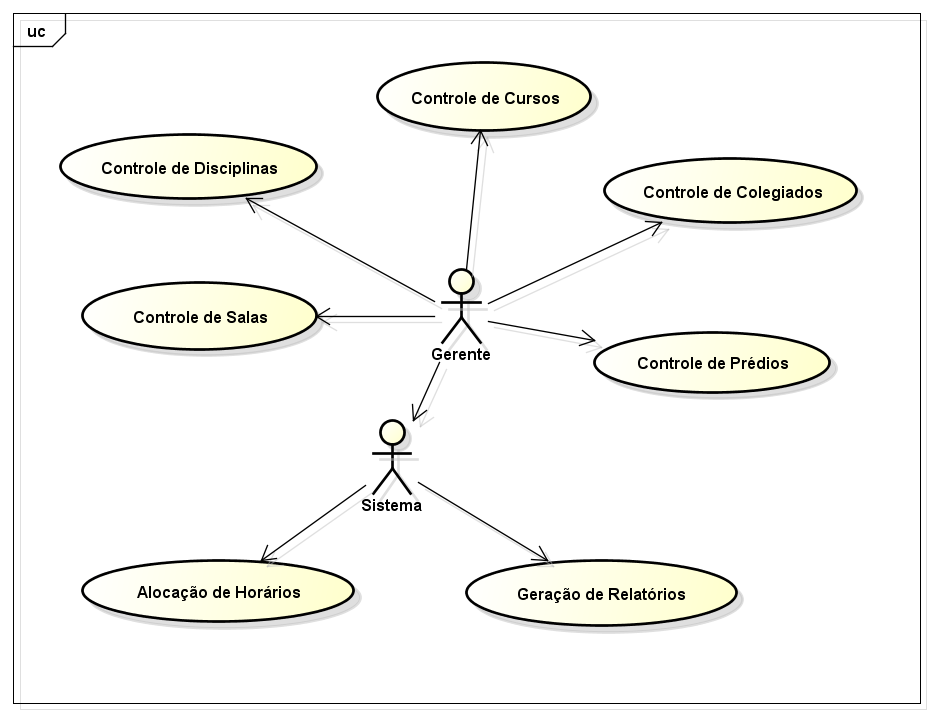
\includegraphics[scale=0.5]{imagens/diagramaCasoUso.png}
\\ \textbf{\footnotesize Fonte: Desenvolvido pelo autor}
\end{figure}

\subsecao{Diagrama de Entidade Relacionamento}


Arrumar referencia \par

Por se tratar de uma aplicação de banco de dados, a modelagem de dados foi também construída. Segundo Elmasri & Navathe (2005) a modelagem conceitual é uma fase muito importante no planejamento de uma aplicação de um banco de dados bem sucedida. Ainda segundo Elmasri & Navathe (2005), o modelo relacional representa o banco de dados como uma coleção de relações. Informalmente, cada relação se parece com uma tabela de valores.


Na Figura XXX tem-se o diagrama para o esquema do banco de dados relacional do sistema. \par
Breve explicação de cada tabela? \par



\begin{figure}[!htb]
\caption[Diagrama de Entidade Relacionamento]{Diagrama de Entidade Relacionamento}
\label{fig:figura1}
\centering
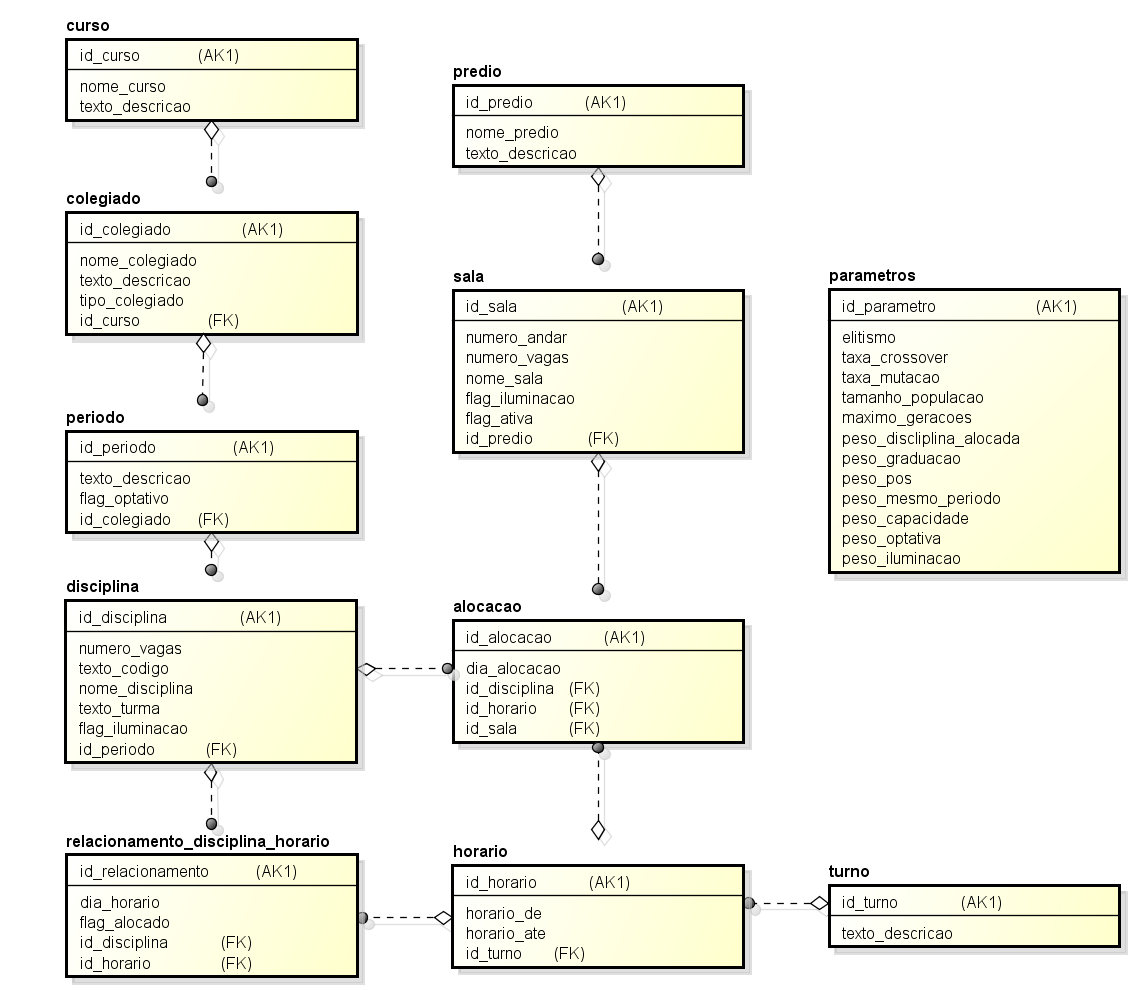
\includegraphics[scale=0.55]{imagens/diagramaEntidadeRelacionamento.png}
\\ \textbf{\footnotesize Fonte: Desenvolvido pelo autor}
\end{figure}

\subsecao{Diagramas de classe}

Quando terminar o codigo revisar.\par

Segundo Booch et al. (2001), Diagrama de Classes demonstram a estrutura estática
das classes de um sistema, onde estas representam as “coisas” que são gerenciadas pela
aplicação modelada. Ainda segundo Booch et al. (2001), uma classe num diagrama pode
ser diretamente implementada utilizando-se uma linguagem de programação orientada a
objetos, no caso deste trabalho, a Linguagem Java.
A partir da Figura 3.7 pode-se observar as classes manipuladores do sistema. Elas
estão identificadas, descritas com seus métodos e relacionadas entre si. Geralmente um
sistema possui mais de um diagrama, pois nem todas se encaixam em um diagrama
específico.

\begin{figure}[!htb]
\caption[Diagrama de componetes do sistema xxx]{Diagrama de componetes do sistema xxx}
\label{fig:figura1}
\centering
\includegraphics{images/diagramaComponentes.png}
\\ \textbf{\footnotesize Fonte: Desenvolvido pelo autor}
\end{figure}

\secao{Algoritimo Genético}


O primeiro passo a ser dado para o desenvolvimento do algoritimo é o pleno conhecimento do problema e a ligação entre os termos utilizados na biologia com os itens do problema proposto anteriormente. Foram utilizadas varias fontes para o desenvolvimento do trabalho, porem foram feitas modificação para que o modelo tratado por outros autores funcionasse como necessario.\par

Para o melhor entendimento dos passos tomados durante a interpretação do problema e da sua ligação com o algoritmo genetico será criado um pequeno ambiente de alocação. Este ambiente contem as seguintes propriedades, três salas, seis horarios, sete dias da semana, cinco discplinas e nove relacionamentos de obrigatoriedade entre discplina e horário.\par

\begin{figure}[!htb]
\caption[Representação do ambiente]{Representação do ambiente}
\label{fig:figura1}
\centering
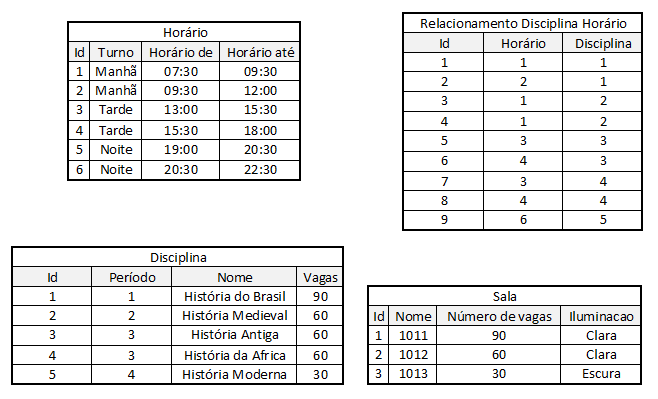
\includegraphics[scale=0.8]{imagens/representacaoAmbiente.png}
\\ \textbf{\footnotesize Fonte: Desenvolvido pelo autor}
\end{figure}

\subsecao{Individuo}

Alguns trabalhos tratam cromossomos e inidviduos pela mesma representação biologica, neste caso cromosso neste trabalho o termo cromossomo se refere a segquencia de genes e o termo Indiviuo será a combinação de cromossomo e fitness.\par

O termo Gene representa uma combinação de quatro variaveis Sala, Dia da Semana, Horario, e o relacionamento entre Disciplina Horario. As três primeiras variaveis são fixas e não podem ser nulas pois o conjunto de Genes forma um cromossomo que é a alocação de todas as discplinas em horarios diferentes.\par

Um Gene com o relacionamento Disciplina Horario igual a nulo, representa um horario vago, como exemplo podemos descrever a seguinte situação, mostra que nos determinados parametros não existe nenhuma sala alocada.\par

\begin{figure}[!htb]
\caption[Representação Gene]{Representação Gene}
\label{fig:figura1}
\centering
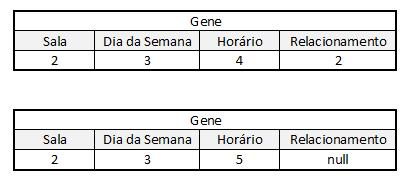
\includegraphics[scale=0.7]{imagens/representacaoGene.png}
\\ \textbf{\footnotesize Fonte: Desenvolvido pelo autor}
\end{figure}

Um cromossomo é uma seguencia de genes o que representa uma alocação completa que engloba todas as salas, todos os dias da semana, e todos os horarios disponiveis para alocação de disciplinas. Uma vez que este valor não é variavel temos um cromossomo com um valor fixo, que serão inseridos os horarios disponiveis para alocação das disciplinas. O tamanho do cromossomo é medido pela seguinte formala (Número de Salas * Número de Horários * Número de dias da semana) neste ambiente o valor é igual a 210 Genes que compoe o cromossomo. A representação binaria do cromossomo se deve ao item relacionamento do Gene estar preenchido ou não 1 para preenchido e zero para nulo. A representação gráfica do cromossomo apenas id do relacionamento para uma melhor visualização.\par


\begin{figure}[!htb]
\caption[Representação Cromossomo]{Representação Cromossomo}
\label{fig:figura1}
\centering
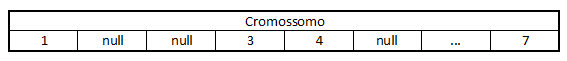
\includegraphics[scale=0.8]{imagens/representacaoCromossomo.png}
\\ \textbf{\footnotesize Fonte: Desenvolvido pelo autor}
\end{figure}

Por fim individuo é a combinação do cromossomo e a pontuação adquirida após a execuação do metodo de calculo de fitness.

\subsecao{Populacao}

População é o conjunto de individuos

Populacao Inicial  escrever como funciona o random

Nova População

Melhor

\subsecao{Operadores Geneticos}
elitismo
crossover
mutacao

\subsecao{Definição da função objetivo}
Somatorio disso

Para o calculo do fitness foram definidos pesos para modelagem da função, estes pesos podem ser configurados de acordo com a necessidade da alocação.

Graduação alocada ganha 05 de peso

Pós graduação alocada ganha 03 de peso

Periodos na mesma sala cada um ganha 05 de peso * o numero do periodo

Quanditadade de vagas igual a da sala 05 de peso

não optativa ganha 5

optativa ganha 3

iliminacao atendida 5

Criar a função matematica com as legendas conforme o trabalho 117.pdf

Falar o numero de salas, o numero de horarios, o numero de curos o numero de colegiados o numero de periodos o numero de disciplinas para cada colegiado.......

restrições 


falar um pouco das restrições e enumeralas

As disciplinas não podem ser alocadas em horarios direfentes dos que já foram pré definidos pelo colegiado.

As discplinas devem ter apenas a quantidade de alocações necessarias.

As disciplinas devem respeitar a capacidade da sala.

As diciplinas não optativas tem preferencia de alcação na mesma sala.

Preferencias por salas claras ou escuras

Restrição 1 


Fitness

Para se iniciar o calculo do fitness são verificados todos os horarios já alocados somando os pesos se adequados.

para cada gene

se tem horario alocado 

horario bate

capacidade da turma

turma graduacao

optativa

iluminacao

soma tudo

fim se tem alocação

soma tudo

fim para cada gene

Calculo do fitness01 somatatoriox100/colocar algum valor  para dividir não sei ainda

calculo fitness02 penaliza disciplinas com mais alocação do que se deve

para cada gene 

para cada disciplina 

soma

fim

Calculo fitness02 -= fitnes01 x (1 - (total alocados - total necessario/ dividir pelo numero possivel de alocações))
fim

calculo fitness03 penalidade por capacidade

para cada gente

se a sala tiver capacidade diferente

fim

calculo fitness03 = fitness02 x (1 - (numero de erros /  numero de possiveis alocações )))


calculo fitness04 preferencias clara ou escura

para cada gene 

se tiver com o optativo errado 

fim	

calculo fitness04 = fitness03 x (1 - (numero de erros /  numero de possiveis alocações )))


O fitness04 é o resultado final

\subsecao{Seleçao por torneio}




%\capitulo{RESULTADOS E DISCUSSÕES}

\capitulo{CONCLUSÃO}

\iniciocapitulo
Discussão dos resultados obtidos na pesquisa, onde se verificam as observações pessoais do autor. Poderá também apresentar sugestões de novas linhas de estudo. A conclusão deve estar de acordo com os objetivos do trabalho. A conclusão não deve apresentar citações ou interpretações de outros autores.

\secao{Trabalhos futuros}

Criar um DW para geração dos relatorios de acordo com a dimensão escolhida.

Utilização de outros algoritimos para a resolução do problema ex. algoritimos evolutivos formiga entre outros.

%\referencias{referencias}
%\capitulo{APÊNDICES}

\end{document}